\documentclass[fleqn,usenatbib]{mnras}
\usepackage[T1]{fontenc}
\usepackage{mathptmx}
\usepackage{graphicx,booktabs,amsmath,amssymb,array,etoolbox}
\usepackage{microtype}
\usepackage{hyperref}
\hypersetup{colorlinks=true,linkcolor=blue,citecolor=blue,urlcolor=blue}
\newcommand{\lcdm}{$\Lambda$CDM}
\newcommand{\hunit}{\mathrm{km\,s^{-1}\,Mpc^{-1}}}
\newcommand{\rd}{r_{\rm d}}
\title[Multi-probe cosmology in September 2026]{Multi-probe cosmology in September 2026: a reproducible MCMC analysis of Planck, ACT, DESI and DES-Dovekie}
\author[Research draft]{Prepared for Nic Ross\\
\small Computational research draft; independent scientific review pending}
\date{7 September 2026. Public-data audit completed 4 September 2026.}
\pubyear{2026}
\makeatletter
\gdef\@journal{\textbf{MNRAS-style research draft}\hfill 7 September 2026}
\apptocmd{\ps@headings}{\def\@oddfoot{\hfill\small Research draft (2026)}\def\@evenfoot{\small Research draft (2026)\hfill}}{}{}
\apptocmd{\ps@titlepage}{\def\@oddfoot{\small Prepared for scientific review\hfill}\def\@evenfoot{\hfill\small Prepared for scientific review}}{}{}
\makeatother
\begin{document}
\pagestyle{headings}
\label{firstpage}
\pagerange{\pageref{firstpage}--\pageref{lastpage}}
\maketitle
\begin{abstract}
We present newly executed cosmological parameter inference using public CMB,
baryon acoustic oscillation (BAO) and Type Ia supernova likelihoods. Our baseline
combines Planck 2018 large-scale temperature and polarization, ACT DR6
foreground-marginalized spectra, DESI DR2 galaxy BAO, the July 2026 Ly$\alpha$
Alcock--Paczynski plus BAO distance measurement, and the recalibrated
DES-Dovekie supernova sample. We fit spatially flat \lcdm, constant-$w$ CDM and
Chevallier--Polarski--Linder (CPL) dark energy, varying the six standard CMB
parameters and instrumental calibration parameters. @@ABSTRACT_RESULTS@@
Four independent Markov chains per model sample a numerical theory surrogate;
retained draws are recalculated with CAMB and importance-corrected to the direct
likelihood. We report both chain convergence and correction efficiency.
Pantheon+ and the previous Ly$\alpha$ BAO measurement provide sensitivity tests.
The results are conditional on fixed neutrino mass and standard early-time
physics. Recent weak-lensing, cluster, SPT and distance-scale measurements are
discussed as external comparisons, rather than incorporated through unvalidated
products of published parameter estimates.
\end{abstract}
\begin{keywords}
cosmological parameters -- dark energy -- cosmic background radiation --
large-scale structure of Universe -- supernovae: general -- methods: statistical
\end{keywords}

\section{Introduction}
The present cosmological data set probes the same expansion history in markedly
different ways. CMB acoustic structure calibrates the physical matter densities
and the sound horizon. BAO traces radial and transverse distances relative to
that ruler. Standardized supernovae measure the relative luminosity-distance
relation. Agreement among these observables is a stronger test than agreement
among parameter values obtained after imposing \lcdm\ separately.

Two recent changes motivate a fresh calculation. DES-Dovekie updates the
cross-survey photometric calibration and light-curve analysis of DES-SN5YR
\citep{Dovekie}. DESI's July 2026 Ly$\alpha$ analysis adds information from the
Alcock--Paczynski effect to its BAO distances \citep{DESI2026}. Both are relevant
to claims of evolving dark energy. Meanwhile, ACT DR6 provides precise CMB
polarization data that complement Planck \citep{ACT2025,ACTextended}.

This paper answers a deliberately specified statistical question: what do these
public likelihood products imply within three nested flat cosmological models?
It is a reanalysis of released summary likelihoods, not a new reduction of
detector maps, galaxy catalogues or supernova light curves. Table~\ref{tab:data}
states the fitted scope. Other major contemporary experiments are assessed in
Section~\ref{sec:context}; they are not silently treated as independent Gaussian
parameter priors. All tables identified as our results derive from calculations
executed for this draft.

\begin{table*}
\centering
\caption{Data scope and treatment. CMB bandpowers retain their released covariance and windows. Counts refer to retained likelihood entries, not numbers of independent sky modes.}
\label{tab:data}
\begin{tabular}{p{0.19\textwidth}p{0.40\textwidth}p{0.34\textwidth}}
\toprule
Probe & Fitted information & Treatment and limitation\\
\midrule
Planck 2018 & 252 Plik-lite bins: TT to $\ell=1000$, TE/EE to 600; Commander TT and SimAll EE at $2\leq\ell\leq29$ & Foregrounds marginalized upstream; shared CMB calibration with Gaussian $0.25$ per cent prior.\\
ACT DR6 & 135 TT/TE/EE bandpowers, $600\leq\ell_{\rm eff}\leq6500$ & Supplied windows through $\ell=8501$; polarization efficiency varied.\\
DESI DR2 & 13 BAO distances from $z=0.295$ to 2.33 & Full released covariance; no additional SDSS/DESI DR1 duplication.\\
DESI Ly$\alpha$ 2026 & Joint $D_M/\rd,D_H/\rd$ at $z=2.33$ & Replaces older Ly$\alpha$ pair; rounded Gaussian summary from equation (26) of \citet{DESI2026}.\\
DES-Dovekie & 1820 supernovae, total released precision & Individual redshifts; common magnitude offset marginalized.\\
Pantheon+ & 1590 light curves at $z_{\rm HD}>0.01$ & Alternative to Dovekie; full covariance; no Cepheid calibration.\\
Other recent probes & DES Y6, KiDS-Legacy, SPT-3G, lensing reconstruction, clusters, local distances, sirens & Literature context only; no raw likelihood refit in this work.\\
\bottomrule
\end{tabular}
\end{table*}

\section{Cosmological models and likelihoods}
\subsection{Theory and priors}
We assume spatial flatness, adiabatic scalar perturbations, a power-law
primordial spectrum, standard recombination and general relativity. CAMB
\citep{CAMB} calculates the expansion, lensed spectra, sound horizons and linear
matter fluctuation amplitude. The varied CMB parameters are
$\omega_b=\Omega_bh^2$, $\omega_c=\Omega_ch^2$, $100\theta_\star$,
$\ln(10^{10}A_s)$, $n_s$ and $\tau$. We derive $H_0$, $\Omega_m$, $\rd$,
the cosmic age, $\sigma_8$ and $S_8=\sigma_8\sqrt{\Omega_m/0.3}$.
The sum of neutrino masses is fixed to $0.06$ eV, with one massive species and
$N_{\rm eff}=3.046$. Helium follows CAMB's BBN consistency relation; no
primordial-abundance likelihood is added. Tensors, running and spatial curvature
are fixed to zero, and lensing is not assigned a free phenomenological amplitude.
The primordial pivot is $k=0.05\,\mathrm{Mpc}^{-1}$. Non-linear corrections to
the lensing calculation use CAMB's HMcode-2020 prescription with its default
parameters; no separate baryonic-feedback parameter is fitted.

For \lcdm, $w=-1$. Constant-$w$ CDM adds one parameter. CPL adds two,
\begin{equation}
 \begin{aligned}
 w(a)&=w_0+w_a(1-a),\\
 \frac{\rho_{\rm de}(a)}{\rho_{{\rm de},0}}
 &=a^{-3(1+w_0+w_a)}\exp[-3w_a(1-a)].
 \end{aligned}
\end{equation}
following \citet{CPL,Linder}. The parametrized post-Friedmann treatment permits
crossing $w=-1$. Sampling uses $w_p=w_0+w_a/4$ to reduce correlations; the linear
transformation has unit Jacobian and does not change a flat $(w_0,w_a)$ prior.
This fixed $w_p$ is the value at $z=1/3$, not a data-optimized pivot.

The uniform prior ranges are $\omega_b\in(0.0205,0.0245)$,
$\omega_c\in(0.105,0.135)$, $100\theta_\star\in(1.038,1.044)$,
$\ln(10^{10}A_s)\in(2.8,3.3)$, $n_s\in(0.92,1.03)$,
$\tau\in(0.01,0.12)$, $w_0\in(-2,0)$ and $w_a\in(-3,1)$,
with $w_0+w_a<0$ and CAMB solutions restricted to
$35<H_0/\hunit<100$. We inspect posterior occupancy near these limits.
Instrument parameters are $A_{\rm CMB}\sim\mathcal{N}(1,0.0025^2)$, restricted
to $(0.98,1.02)$, and $P_{\rm ACT}\in(0.9,1.1)$.

\subsection{CMB}
The Planck likelihood combines Plik-lite with the native Commander and SimAll
implementations distributed through Cobaya \citep{Planck2020}. We retain
Plik-lite bins whose upper edges lie below 1000 in TT and 600 in TE and EE,
following the large-scale Planck plus ACT construction. Covariance submatrices
are selected before inversion. ACT DR6 uses the collaboration's
foreground-marginalized TT/TE/EE data \citep{ACT2025}. Its Gaussian term is
\begin{equation}
 -2\ln\mathcal{L}_{\rm ACT}
 = (\boldsymbol d-\boldsymbol W\boldsymbol D_\ell)^T
 C_{\rm ACT}^{-1}(\boldsymbol d-\boldsymbol W\boldsymbol D_\ell)
 +\mathrm{const.},
\end{equation}
where $D_\ell=\ell(\ell+1)C_\ell/(2\pi)$. Theory is divided by
$A_{\rm CMB}^2$ and, for ACT TE and EE, additionally by $P_{\rm ACT}$ and
$P_{\rm ACT}^2$. Low-multipole likelihoods retain their non-Gaussian form.

There remains TT multipole overlap between Planck and ACT at
$600\lesssim\ell\lesssim1000$; we follow the public combination's approximation
of neglecting cross-experiment covariance. Foreground marginalization, these
cuts, SimAll rather than SRoll2, and the omission of reconstructed CMB-lensing
likelihoods distinguish our results from the full published P-ACT combinations.
We have not reproduced the multi-frequency foreground analysis or independently
validated its compression for every dark-energy extension.

\subsection{BAO and the 2026 Ly$\alpha$ update}
We use the DESI DR2 mean vector and covariance \citep{DESI2025}, comparing to
\begin{equation}
 D_H=\frac{c}{H(z)},\quad D_M=(1+z)D_A,\quad
 D_V=[zD_M^2D_H]^{1/3},
\end{equation}
in units of the CAMB drag-epoch sound horizon. To include the new full-shape
Ly$\alpha$ information, we replace the old pair at $z=2.33$ with
\begin{align}
 D_M/\rd&=39.32\pm0.33,\\
 D_H/\rd&=8.600\pm0.066,\qquad \rho=0.225.
\end{align}
The covariance is reconstructed from these published rounded errors and
correlation \citep{DESI2026}. This uses the released distance-level result; it
does not refit Ly$\alpha$ correlation functions. Appending this pair to the
original BAO pair would double-count the same forest data. The original
BAO-only pair is retained for a replacement sensitivity test.

\subsection{Supernovae}
DES-Dovekie supplies a total \emph{precision} matrix in packed upper-triangular
form, rather than a covariance requiring a further diagonal statistical term
\citep{Dovekie}. We reconstruct it without changing the release ordering.
Pantheon+ uses the total covariance after applying $z_{\rm HD}>0.01$
\citep{Pantheon,PantheonData}; repeated light curves are retained with their
correlations. These compilations are fitted as alternatives because they share
objects and calibration information.

Using both the Hubble-diagram and heliocentric redshifts, the model modulus is
\begin{equation}
 \mu_i=5\log_{10}\!\left[(1+z_{{\rm HD},i})(1+z_{{\rm hel},i})
 D_A(z_{{\rm HD},i})/{\rm Mpc}\right]+25.
\end{equation}
For residual vector $\boldsymbol\Delta$, precision $P$ and an uninformative
common magnitude-offset prior, the parameter-dependent marginalized statistic is
\begin{equation}
 \chi^2_{\rm SN}=\boldsymbol\Delta^TP\boldsymbol\Delta
 -\frac{(\boldsymbol 1^TP\boldsymbol\Delta)^2}{\boldsymbol 1^TP\boldsymbol 1}.
\end{equation}
The fixed offset-normalization term cancels between models using the same
sample. No SH0ES absolute calibration or independent Gaussian $H_0$ constraint
enters these fits. Supernovae alone therefore do not measure $H_0$ here.

\section{Computation and validation}\label{sec:computation}
Direct theory evaluation through the ACT window support is expensive. We fit a
local cubic polynomial to a bank of @@NTRAIN@@ CAMB predictions in eight
cosmological coordinates. The approximation includes spectra and distance
predictions. A 100-node log-redshift interpolation accelerates the supernova
term while retaining its full quadratic form. This is numerical interpolation
of a smooth prediction, not statistical replacement of the supernova data by
100 independent objects.

Each model is sampled with four separately seeded Metropolis chains. Proposal
covariances and scales adapt during @@WARMUP@@ discarded steps and are frozen
for @@DRAWS@@ production steps per chain. We inspect trace behaviour,
rank-normalized folded/split $\widehat R$, bulk and tail effective sample sizes
\citep{Rhat}. Convergence of the proposal posterior alone does not establish
accuracy of cosmological constraints.

We therefore select draws across all four chains, calculate their spectra and
individual-supernova distances with CAMB, and apply
\begin{equation}
 u_i=\exp[\ln\mathcal L_{\rm direct}(\theta_i)
                 -\ln\mathcal L_{\rm surrogate}(\theta_i)],\quad
 \tilde u_i=\frac{u_i}{\sum_j u_j}.
\end{equation}
This importance correction follows the general approach described by
\citet{LewisBridle}. The final parameter tables and credible regions use these
direct-likelihood weights. We record $N_{\rm IS}=1/\sum_i\tilde u_i^2$ and
Pareto-tail diagnostics separately from MCMC ESS. Raw surrogate chains,
retained direct evaluations and both log densities are included in the
reproducibility bundle. @@DIAGNOSTICS_TEXT@@

@@DIAGNOSTICS_TABLE@@

CAMB version 2.0.4 is used with Recfast recombination, lensed spectra through
$\ell=8501$, lens-potential accuracy 1, accuracy boosts 1.2 and a lens-output
margin of 700. A higher-accuracy calculation uses boosts 2, lens-potential
accuracy 2 and margin 1200. @@ACCURACY_TEXT@@ These checks address numerical
error; they do not remove physical modelling or inter-survey calibration
uncertainty. The Gaussian high-$\ell$ terms and SN residuals are inspected
separately. Because low-$\ell$ terms are non-Gaussian and contain likelihood
offsets, their sum is not assigned a naive global $\chi^2$ goodness-of-fit
probability.

\section{Results}\label{sec:results}
\subsection{Parameter constraints}
@@RESULTS_TEXT@@
@@PARAMETER_TABLE@@

\begin{figure*}
\centering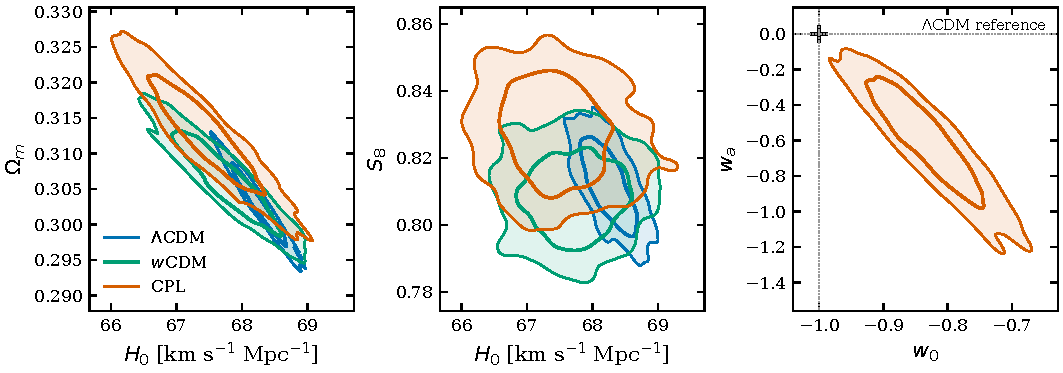
\includegraphics[width=\textwidth]{posterior.pdf}
\caption{Direct-CAMB importance-corrected posterior constraints. Contours enclose
68 and 95 per cent of the plotted two-dimensional densities. In the CPL panel,
the cross marks $(w_0,w_a)=(-1,0)$. The displayed dark-energy covariance must be
considered jointly; separate one-dimensional exclusions are not independent
significance tests.}
\label{fig:posterior}
\end{figure*}

\subsection{Fit quality and model comparison}
@@MODEL_COMPARISON_TEXT@@
@@MODEL_TABLE@@
We report an AIC-like penalized-deviance diagnostic,
$\Delta D+2\Delta k$, for the nested models with unchanged data and calibration
treatment. It is not a Bayesian evidence calculation. The common SN-offset
normalization cancels, and the additional cosmological parameter counts are one
and two for constant-$w$ and CPL. We do not convert $\sqrt{\Delta D}$ into a
Gaussian significance for a two-parameter extension. Neither a posterior
credible contour nor this diagnostic establishes a discovery of a physical
dark-energy field.

\begin{figure*}
\centering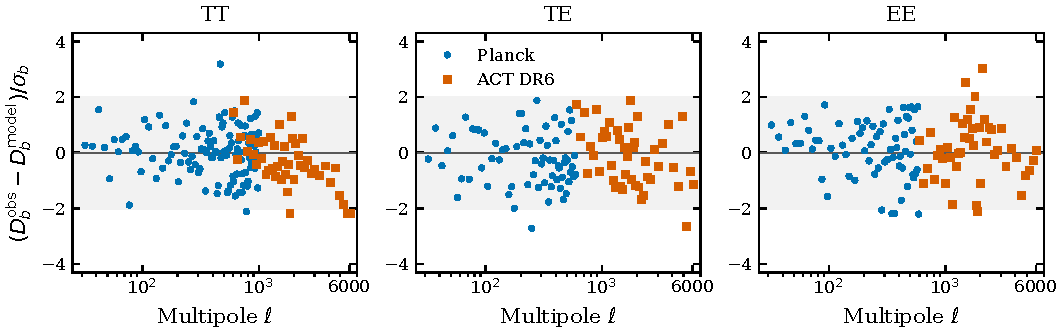
\includegraphics[width=\textwidth]{cmb_residuals.pdf}
\caption{CMB bandpower residuals at the direct-CAMB local \lcdm\ fit, divided
by the released diagonal errors. Blue circles denote retained Planck bins and
orange squares ACT DR6. The shaded region spans two diagonal standard errors.
Bandpower correlations enter the likelihood; the displayed points are not
independent unit-variance tests.}
\label{fig:cmb}
\end{figure*}

\begin{figure*}
\centering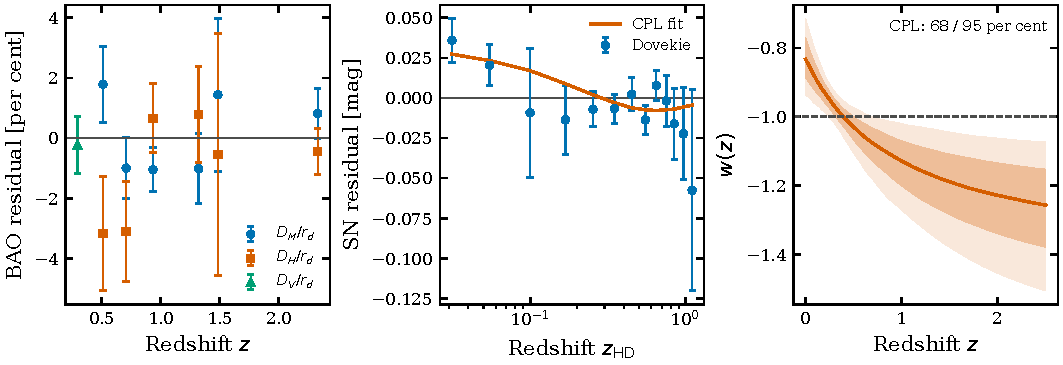
\includegraphics[width=\textwidth]{distance_tests.pdf}
\caption{Distance and expansion-history tests. BAO residuals include the updated
Ly$\alpha$ distance pair; the baseline \lcdm\ prediction defines the reference.
The supernova display uses generalized least-squares bins of Dovekie residuals,
with covariance between bins retained in their construction; these points are
for visualization, while the likelihood uses all 1820 objects. CPL $w(z)$ bands
are posterior intervals within the stated parametrization.}
\label{fig:distances}
\end{figure*}

\subsection{Data-choice sensitivity}
@@SENSITIVITY_TEXT@@
These replacement tests preserve the CMB treatment and cosmological priors.
They assess sensitivity, not the independence of overlapping surveys. When
importance weights become concentrated, the resulting effective sample count
limits the precision of the comparison; a small weight ESS is not repaired by
quoting the much larger original chain length.

\section{Relation to the wider data landscape}\label{sec:context}
The following are published measurements, not new joint fits performed here.
DES Y6 reports $S_8=0.789\pm0.012$ in flat \lcdm\ and finds a 1.8$\sigma$
full-parameter difference from its Planck--ACT--SPT reference, versus
2.6$\sigma$ when projected onto $S_8$ \citep{DESY6}. KiDS-Legacy gives
$S_8=0.815^{+0.016}_{-0.021}$, compatible with its Planck comparison
\citep{KiDS}. The differing calibrations and nuisance treatments caution
against describing a unique, experiment-independent ``$S_8$ tension''.
Our inferred $S_8$ provides a conditional comparison, not a new weak-lensing
measurement or a growth-versus-geometry consistency fit.

SPT-3G D1 is a major further CMB test \citep{SPT}; adding it requires its
likelihood, calibration and overlap prescription. Reconstructed ACT/Planck
CMB lensing \citep{Lensing} tests growth and helps break geometric degeneracies,
but shares sky information with primary CMB data. Cluster abundance, including
eROSITA \citep{eROSITA}, adds mass-calibration, selection and non-linear
modelling requirements. We do not replace these analyses with one-dimensional
$S_8$ Gaussian likelihoods in extended cosmologies.

The Local Distance Network reports
$H_0=73.50\pm0.81\,\hunit$ \citep{DistanceNetwork}. Our inverse-distance-ladder
constraints can be compared with that result, but a formal tension significance
would require accounting for shared SN information and the full model
dependence. The new GWTC-5.0 standard-siren analysis provides an independent
distance-scale test with population and selection modelling
\citep{GWTC5}; current broad siren constraints do not by themselves discriminate
the two distance scales decisively.

Other compilations, including Union3, and cosmic chronometers merit future
replacement tests with their intended likelihood conventions. Older overlapping
BAO releases are not automatically additional information. Validated cosmological likelihoods from Euclid, Rubin and Roman would extend
this analysis as they become available. A global analysis of all probes would additionally require their
shared-volume and calibration covariances.

\section{Discussion and conclusions}
@@CONCLUSIONS_TEXT@@
The essential limitation is model scope. Flatness, fixed neutrino mass and
standard early-time physics are assumptions here. These chains cannot establish
curvature limits, neutrino-mass bounds, early dark energy, modified gravity or
the origin of any discrepancy. Late-time CPL freedom alone is not a general
solution to a distance-scale mismatch, and $w_0$--$w_a$ is an empirical
description rather than a unique microphysical theory.

Before journal submission, an independent implementation should verify the
likelihood conventions and compare alternative CMB reductions and full
foreground treatments. Adding reconstructed lensing, SPT and galaxy-lensing
likelihoods with validated cross-covariances is the natural next extension.
The attached data, code, weighted draws and diagnostics make the present
calculation inspectable and reproducible.

\section*{Data and code availability}
The accompanying archive contains the pinned public likelihood inputs, their
source URLs and SHA-256 hashes, the executed Python pipeline, random seeds,
surrogate and direct-likelihood samples, numerical diagnostics, figure code and
this manuscript's \LaTeX\ source. Observational data and upstream likelihoods
remain the work of their respective collaborations. No proprietary or mock
observational data are used. The analysis was executed on 4--7 September 2026.

\section*{Acknowledgements and draft status}
This computational draft and its code were generated with ChatGPT at Nic
Ross's request. The named recipient has not independently certified the
analysis, and no authorship or institutional endorsement is asserted. We thank
the survey collaborations and software authors for public data and likelihoods.
This document has not been submitted to or accepted by MNRAS.

\bibliographystyle{mnras}
\bibliography{references}
\clearpage
\onecolumn
\appendix
\section{Chain diagnostics}
\begin{minipage}{\textwidth}
\makeatletter\def\@captype{figure}\let\@makecaption\SFB@makefigurecaption\makeatother
\centering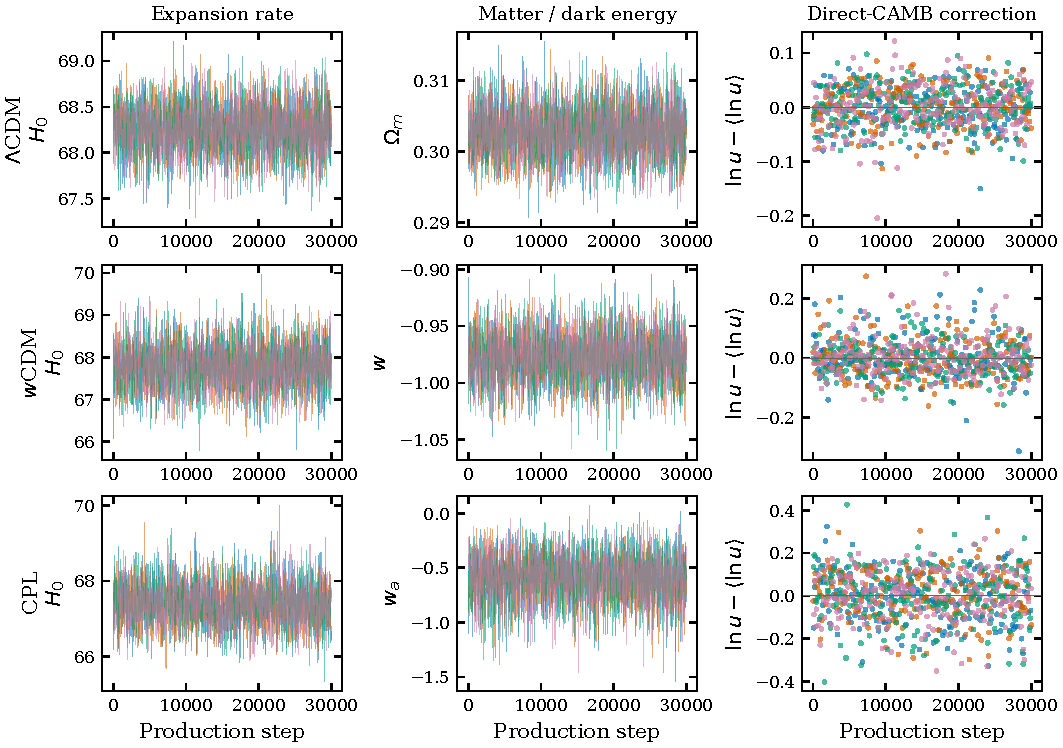
\includegraphics[width=\textwidth]{chains.pdf}
\caption{Production-chain traces and direct-likelihood importance corrections.
Different colours denote independent chains. Display thinning is used only to
keep the figure legible; diagnostic calculations use the full stored chains.}
\label{fig:chains}
\end{minipage}
\label{lastpage}
\end{document}
